\documentclass{article}

\usepackage{graphicx} % Required to insert images
\graphicspath{ {./} }
\usepackage{amsmath,eqnarray,easybmat} % Required for Math Stuff
\usepackage{enumerate,textpos}
\usepackage{algorithmic,algorithm} % Alg packages
\usepackage{amssymb,amsthm}
\usepackage{hyperref,color,fullpage}
\usepackage{wrapfig}
\usepackage{csquotes}
\usepackage[]{natbib}
\usepackage{bm}
\usepackage{titlesec}
\usepackage{multicol}
\usepackage{ulem}
\usepackage{caption}
\usepackage{subcaption}
\usepackage{flushend}
\usepackage{listings}
\usepackage{float}

%----------------------------------------------------------------------------------------
%	NEW COMMANDS
%----------------------------------------------------------------------------------------

\let\wh\widehat
\let\bs\boldsymbol

\renewcommand{\algorithmicrequire}{\textbf{Input:}}
\renewcommand{\algorithmicensure}{\textbf{Output:}}

\renewcommand{\hat}{\widehat}

% special characters

\newcommand{\removed}[1]{}

\newcommand{\cD}{\mathcal{D}}
\newcommand{\cF}{\mathcal{F}}
\newcommand{\cP}{\mathcal{P}}
\newcommand{\cE}{\mathcal{E}}
\newcommand{\cU}{\mathcal{U}}
\newcommand{\cV}{\mathcal{V}}
\newcommand{\cX}{\mathcal{X}}
\newcommand{\cY}{\mathcal{Y}}
\newcommand{\cO}{\mathcal{O}}
\newcommand{\cM}{\mathcal{M}}


\newcommand{\bE}{\mathbb{E}}
\newcommand{\R}{\mathbb{R}}
\newcommand{\bP}{\mathbb{P}}
\newcommand{\bZ}{\mathbb{Z}}

\newcommand{\0}{\mathrm{0}}
\newcommand{\1}{\mathrm{1}}

\renewcommand{\a}{\mathrm{a}}
\newcommand{\A}{\mathrm{A}}
\newcommand{\hA}{\widehat{\mathrm{A}}}
\newcommand{\B}{\mathrm{B}}
\newcommand{\hB}{\widehat{\mathrm{B}}}
\renewcommand{\b}{\mathrm{b}}
\renewcommand{\c}{\mathrm{c}}
\newcommand{\C}{\mathrm{C}}
\renewcommand{\d}{\mathrm{d}}
\newcommand{\D}{\mathrm{D}}
\newcommand{\tC}{\tilde{\C}}
\newcommand{\e}{\mathrm{e}}
\newcommand{\E}{\mathrm{E}}
\newcommand{\f}{\mathrm{f}}
\newcommand{\g}{\mathrm{g}}
\newcommand{\G}{\mathrm{G}}
\newcommand{\h}{\mathrm{h}}
\renewcommand{\H}{\mathrm{H}}
\newcommand{\cH}{\mathcal{H}}
\renewcommand{\i}{\mathrm{i}}
\newcommand{\I}{\mathrm{I}}
\renewcommand{\j}{\mathrm{j}}
\renewcommand{\k}{\mathrm{k}}
\newcommand{\K}{\mathrm{K}}
\newcommand{\m}{\mathrm{m}}
\newcommand{\M}{\mathrm{M}}
\newcommand{\n}{\mathrm{n}}
\newcommand{\N}{\mathrm{N}}
\renewcommand{\o}{\mathrm{o}}
\newcommand{\p}{\mathrm{p}}
\renewcommand{\P}{\mathrm{P}}
\newcommand{\q}{\mathrm{q}}
\newcommand{\Q}{\mathrm{Q}}
\renewcommand{\r}{\mathrm{r}}
\newcommand{\s}{\mathrm{s}}
\renewcommand{\S}{\mathrm{S}}
\renewcommand{\t}{\mathrm{t}}
\newcommand{\T}{\mathrm{T}}
\newcommand{\bT}{\mathbb{T}}
\renewcommand{\u}{\mathrm{u}}
\newcommand{\U}{\mathrm{U}}
\renewcommand{\v}{\mathrm{v}}
\newcommand{\V}{\mathrm{V}}
\newcommand{\w}{\mathrm{w}}
\newcommand{\W}{\mathrm{W}}
\newcommand{\x}{\mathrm{x}}
\newcommand{\X}{\mathrm{X}}
\newcommand{\hX}{\widehat{\mathrm{X}}}
\newcommand{\y}{\mathrm{y}}
\newcommand{\Y}{\mathrm{Y}}
\newcommand{\hY}{\widehat{\mathrm{Y}}}
\newcommand{\z}{\mathrm{z}}
\newcommand{\Z}{\mathrm{Z}}
\newcommand{\Cxemp}{{\mathrm{C}}_{x,t}}
\newcommand{\Cyemp}{{\mathrm{C}}_{y,t}}



\newcommand{\norm}[1]{\left\| #1 \right\|}
\newcommand{\abs}[1]{\rvert #1 \lvert}
\newcommand{\var}[1]{\operatorname{var}\left(#1\right)}
\newcommand{\pr}[1]{\operatorname{Pr}\{#1\}}
\renewcommand{\log}[1]{\operatorname{log}\left(#1\right)}
\renewcommand{\exp}[1]{\operatorname{exp}\left(#1\right)}
\newcommand{\trace}[1]{\textrm{Tr}\left(#1\right)}
\newcommand{\diag}[1]{\operatorname{diag}\left(#1\right)}
\newcommand{\rank}[1]{\operatorname{Rank}\left(#1\right)}
% colors
\newcommand{\red}[1]{{\color{red}{#1}}}
\newcommand{\blue}[1]{{\color{blue}{#1}}}
\newcommand{\gray}[1]{{\color{gray}{#1}}}
\newcommand{\green}[1]{{\color{green}{#1}}}


\newcommand{\expectation}[2]{\mathbb{E}_{#1}\left[#2\right]}
\newcommand{\expect}[1]{\mathbb{E}\left[#1\right]}
\newcommand{\grad}{\triangledown}

\newcommand{\minimize}[3]{
\begin{aligned}
& \underset{#1}{\textrm{minimize:}}
& & #2 \\
& \textrm{subject to:}
& &  #3
\end{aligned}
}

\newcommand{\maximize}[3]{
\begin{aligned}
& \underset{#1}{\textrm{maximize}}
& & #2 \\
& \textrm{subject to}
& &  #3
\end{aligned}
}

\newcommand{\argmax}[4]{
\begin{aligned}
& #4 := \underset{#1}{\textrm{argmax}}
&& #2 \\
& \textrm{subject to}
&&  #3
\end{aligned}
}

\newcommand{\argmin}[4]{
\begin{aligned}
& #4 := \underset{#1}{\textrm{argmin}}
&& #2 \\
& \textrm{subject to}
&&  #3
\end{aligned}
}

\newcommand{\sig}[2]{\sigma_{#1}\left(#2\right)}
\newcommand{\sigh}[2]{\hat{\sigma}_{#1}\left(#2\right)}
\def\infinity{\rotatebox{90}{8}}

\newcommand{\inner}[2]{\left\langle#1,#2\right\rangle}

\newtheorem{theorem}{Theorem}[section]
\newtheorem{lemma}[theorem]{Lemma}
\newtheorem{prop}[theorem]{Proposition}
\newtheorem{claim}[theorem]{Claim}
\newtheorem{cor}[theorem]{Corollary}
\newtheorem{conj}[theorem]{Conjecture}


\begin{document}
\title{Non-negative matrix factorization with smoothness and sparse penalties}
\author{Teodor Marinov, Matthew Francis-Landau, Ryan Cotterell}
\date{}

\maketitle
\section{Problem formulation}
In this project we consider a variant of the non-negative matrix factorization problem (NMF)~\cite{lee2001algorithms}. The basic NMF problem is posed as follows
\begin{equation}\label{problem_1}
  \begin{aligned}
    \minimize{\W\in \mathbb{R}^{d\times k},\H \in \mathbb{R}^{k\times n}}{\norm{\X - \W\H}_F^2}{\W_{i,j} \geq 0,\H_{i,j}\geq 0}
  \end{aligned}
\end{equation}
where $\X\in\mathbb{R}^{d\times n}$ is some data matrix and $k$ is given and fixed. This is a non-convex optimization problem. In~\cite{lee2001algorithms} the authors suggest simple alternating multiplicative updates and claim that the proposed algorithm has a fixed point. In~\cite{gonzalez2005accelerating}, however, it is indicated that the claim is wrong. Another approach to solving problem~\ref{problem_1} is the following algorithm -- initialize $\W_0,\H_0$ randomly, at step $t$ set $W_{t}$ to be the minimizer of
\begin{equation}\label{problem_2}
  \begin{aligned}
    \minimize{\W\in \mathbb{R}^{d\times k}}{\norm{\X - \W_{t-1}\H_{t-1}}_F^2}{\W_{i,j} \geq 0}
  \end{aligned}
\end{equation}
and $\H_t$ to be the minimizer of
\begin{equation}\label{problem_3}
  \begin{aligned}
    \minimize{\H\in \mathbb{R}^{k\times n}}{\norm{\X - \W_{t}\H_{t-1}}_F^2}{\H_{i,j} \geq 0}.
  \end{aligned}
\end{equation}
Proceed to carry out this alternating minimization approach until some stopping criteria is met e.g.\\ $\norm{\W_t\H_t - \W_{t+1}\H_{t+1}}_F^2 < \epsilon$. In~\cite{tropp2003alternating} it is shown that this algorithm is going to have a fixed point. Note that~\ref{problem_2},\ref{problem_3} are now constraint convex-optimization problems so one can choose their favourite method to solve them.
\par
Usually NMF is applied to real-world problems where the $\W$ and $\H$ term have some interpretation -- for example $\X$ can be the Fourier power spectogram of an audio signal where the $m,n$-th entry is the power of signal at time window $n$ and frequency bin $m$. The assumption is that the observed signal is coming from a mixture of $k$ static sound sources. Now each column of $\W$ can be interpreted as the average power spectrum of an audio source and each row of $\H$ can be interpreted as time-varying gain of a source. In practice the number of sources $k$ is not known and we would like to also infer it from the data. This can be done by introducing an additional factor in the optimization problem which indicates the weight of a source in the mixture.
\begin{equation}\label{problem_4}
  \begin{aligned}
    \minimize{\W\in \mathbb{R}^{d\times d}, \Theta \in \mathbb{R}^{d\times d},\H \in \mathbb{R}^{d\times n}}{\norm{\X - \W\Theta\H}_F^2 + \lambda\norm{\Theta}_1}{\W_{i,j} \geq 0,\H_{i,j}\geq 0,\Theta_{i,i} \geq 0,\Theta_{i\neq j} = 0}
  \end{aligned}
\end{equation}
In problem~\ref{problem_4} $\Theta$ is introduced as the weight matrix for the mixture and an $l_1$ penalty is introduced to keep the number of ``active'' sources small. Such a NMF problem has been considered in~\cite{blei2010bayesian} and a Bayesian approach is taken in solving it by specifying distributions over the elements of $\W,\H$ and $\Theta$. In our project we directly try to solve a problem similar~\ref{problem_4} with an additional penalty term which forces the columns of $\W$ to vary smoothly. To conclude the section we present the optimization problem:
\begin{equation}\label{problem_5}
  \begin{aligned}
    \minimize{\W\in \mathbb{R}^{d\times d}, \Theta \in \mathbb{R}^{d\times d},\H \in \mathbb{R}^{d\times n}}{\frac{1}{n}\norm{\X - \W\Theta\H}_F^2 + \lambda\norm{\Theta}_1 + \eta\sum_{i,j}\left(\W_{i,j} - \W_{i+1,j}\right)^2}{\W_{i,j} \geq 0,\H_{i,j}\geq 0,\Theta_{i,i} \geq 0,\Theta_{i\neq j} = 0}
  \end{aligned}
\end{equation}
\section{Algorithm}
TODO: write down the gradients/subgradients of 6,7 and 8
\par
Problem~\ref{problem_5} is not a convex optimization problem, however, if one considers the 3 separate problems
\begin{equation}\label{problem_6}
  \begin{aligned}
    \minimize{\W\in \mathbb{R}^{d\times d}}{\frac{1}{n}\norm{\X - \W\Theta\H}_F^2 + \eta\sum_{i,j}\left(\W_{i,j} - \W_{i+1,j}\right)^2}{\W_{i,j} \geq 0,\H_{i,j}\geq 0}
  \end{aligned}
\end{equation}
\begin{equation}\label{problem_7}
  \begin{aligned}
    \minimize{\Theta \in \mathbb{R}^{d\times d}}{\frac{1}{n}\norm{\X - \W\Theta\H}_F^2 + \lambda\norm{\Theta}_1}{\Theta_{i,i} \geq 0,\Theta_{i\neq j} = 0}
  \end{aligned}
\end{equation}
\begin{equation}\label{problem_8}
  \begin{aligned}
    \minimize{\H \in \mathbb{R}^{d\times n}}{\frac{1}{n}\norm{\X - \W\Theta\H}_F^2}{\H_{i,j}\geq 0}
  \end{aligned}
\end{equation}
each one is a convex optimization problem. What is more the objectives in~\ref{problem_6} and~\ref{problem_7} are smooth and each of the objectives is also strongly convex. The proposed algorithm is now to solve each of the convex optimization problems separately in an alternating fashion. Pseudo code is given in~\ref{alg:meta_nmf}.

\begin{algorithm}[H]
  \caption{Alternating minimization meta algorithm for problem~\ref{problem_5}}
  \label{alg:meta_nmf}
  \begin{algorithmic}
    \REQUIRE $\X,\W_0,\H_0,\Theta_0,\epsilon$
    \ENSURE $\W_T,\H_T,\Theta_T$
    \WHILE{$\norm{\W_{t-1}\H_{t-1}\Theta_{t-1} - \W_t\H_t\Theta_t}_F^2>\epsilon$}
    \STATE{$\argmin{\W\in \mathbb{R}^{d\times d}}{\frac{1}{n}\norm{\X - \W\Theta_t\H_t}_F^2 + \eta\sum_{i,j}\left(\W_{i,j} - \W_{i+1,j}\right)^2}{\W_{i,j} \geq 0,\H_{i,j}\geq 0}{\W_{t+1}}$}
    \STATE{$\argmin{\H \in \mathbb{R}^{d\times n}}{\frac{1}{n}\norm{\X - \W_{t+1}\Theta_{t}\H}_F^2}{\H_{i,j}\geq 0}{\H_{t+1}}$}
\STATE{$\argmin{\Theta \in \mathbb{R}^{d\times d}}{\frac{1}{n}\norm{\X - \W_{t+1}\Theta\H_{t+1}}_F^2 + \lambda\norm{\Theta}_1}{\Theta_{i,i} \geq 0,\Theta_{i\neq j} = 0}{\Theta_{t+1}}$}
  \ENDWHILE
  \end{algorithmic}
\end{algorithm}

The main focus of our project is now to solve each of the problems~\ref{problem_6},\ref{problem_7},\ref{problem_8} by using different algorithms explored in class, comparing our empirical observations with the derived convergence results. The algorithms we choose to compare are Projected Gradient/Subgradient Descent, Simple Dual Averaging and Augmented Lagrangian. For Projected Gradient/Subgradient Descent we both experiment with fixed step size and decreasing step size as $\frac{1}{t}$. We are also going to assume that all the minimizers of the above problems are in some compact set -- it is not hard to imagine that this holds true, for example consider minimizing the objective in~\ref{problem_6}. If we let $\norm{\W}_F$ go to infinity for fixed $\Theta,\H$ and $\X$ the objective is going to go to infinity and thus $\norm{\W}_F$ must be bounded so we can assume that there exists optimal $\W^*$ is in some bounded closed ball with respect to the Frobenius norm. Thus we can restrict our attention on solving the optimization problems on the intersection of closed set with a compact set i.e. a compact set. Thus we can assume the existence of at least one minimizer of each of the optimization problems~\ref{problem_6},\ref{problem_7} and~\ref{problem_8}
\subsection{Subgradients for problems~\ref{problem_6},\ref{problem_7},\ref{problem_8}}
If $f$ denotes the respective objective of problems~\ref{problem_6},\ref{problem_7} and~\ref{problem_8} then gradients and an element of the subdifferential of~\ref{problem_7} is given by
\begin{equation}
  \label{subgrad_6}
  \begin{aligned}
    \nabla f(\W) &= \frac{2}{n} \left(\W\Theta\H - \X\right)\left(\Theta\H\right)^\top + \eta\tilde{\W} \text{ where }\\
    \tilde{\W}_{i,j} &= 2\left(2\W_{i,j} - \W_{i+1,j} - \W_{i-1,j}\right),\\
    \tilde{\W}_{1,j} &= 2\left(\W_{1,j} - W_{2,j}\right),\\
    \tilde{\W}_{d,j} &= 2\left(\W_{d,j} - \W_{d-1,j}\right)
    \end{aligned}
\end{equation}
\begin{equation}
  \label{subgrad_8}
  \begin{aligned}
    \nabla f(\H)  &= \frac{2}{n}\left(\W\Theta\right)^\top\left(\W\Theta\H - \X\right)
  \end{aligned}
\end{equation}
\begin{equation}
  \label{subgrad_7}
  \begin{aligned}
    \left(\frac{2}{n}\W^\top\left(\W\Theta\H-\X\right)\H +\lambda\text{sgn}\left(\Theta \right)\right)\odot\I \in \partial f(\Theta)
  \end{aligned}
\end{equation}
where $\odot$ denotes the Hadamard product and ``sgn'' is the sign function applied element wise to $\Theta$. The derivation in~\ref{subgrad_7} holds because $\Theta$ is always constraint to be a diagonal matrix.
\section{Projected Gradient Descent}
\subsection{Fixed step size}
TODO: include experiments and comment on comparison with the theory
\par
For this part of the project a modified version of \textbf{Algorithm 1} from lecture slides $4$ is used with different choices of fixed step size $\alpha_k$. The difference with the algorithm given in lecture 4 is the stopping criteria -- as already discussed in class checking if the norm of the gradient is close to $0$ will not work well for objectives including $l_1$ penalty term, instead we choose to stop our procedure either after a fixed number of steps (in our experiments this is 200 when solving problems~\ref{problem_6} and \ref{problem_7} and 500 when solving problem~\ref{problem_8}) or if the distance between consecutive iterates becomes less than $\epsilon$ (where $\epsilon$ was set to be in the range $[10^{-4},10^{-5}]$). As discussed in class this is usually not a good stopping criteria unless the objective is differentiable with $L$-Lipschitz continuous derivatives. Luckily both the objectives in~\ref{problem_6} and~\ref{problem_8} are differentiable with Lipschitz continuous gradients which we show now.
\begin{lemma}\label{lem:lipsch_w}
  The objective in problem~\ref{problem_6} is differentiable with $L$-Lipschitz continuous gradients.
\end{lemma}
\begin{proof}
  Denote the objective in problem~\ref{problem_6} by $f(\W)$. Then $\nabla f(\W) = \frac{2}{n} \left(\W\Theta\H - \X\right)\left(\Theta\H\right)^\top + \eta\tilde{\W}$ where $\tilde{\W}_{i,j} = 2\left(2\W_{i,j} - \W_{i+1,j} - \W_{i-1,j}\right),\tilde{\W}_{1,j} = 2\left(\W_{1,j} - W_{2,j}\right), \tilde{\W}_{d,j} = 2\left(\W_{d,j} - \W_{d-1,j}\right)$. With this we have
  \begin{equation}
    \begin{aligned}
      \norm{\nabla f\left(\W_1 - \W_2\right)}_F =  \norm{\frac{2}{n}\left(\left(\W_1-\W_2\right)\Theta\H\right)\left(\Theta\H\right)^\top + \eta\left(\tilde{\W_1}-\tilde{\W_2}\right)}_F \leq \left(\frac{2}{n}\norm{\Theta\H}_F^2+12\eta\right)\norm{\W_1 - \W_2}_F
    \end{aligned}
  \end{equation}
  where we used triangle inequality and bounded each of the $\norm{(\W_1)_{i,1:j} - (\W_2)_{i,1:j}}_F \leq \norm{\W_1 - \W_2}_F$.
\end{proof}
The above lemma shows that the Lipschitz constant for the objective can indeed be very large as it depends on the product $\Theta\H$, however, in practice setting fixed step size $\alpha \leq 0.05$ seems to be in the range $(0,\frac{2}{L})$ which is when convergence for the algorithm is guaranteed. Sadly we can not guarantee strong convexity or strict convexity for the objectives in~\ref{problem_6} and~\ref{problem_8} so the theorem which charaterizes the best convergence rate is Theorem 1.9 in lecture slides 6. From our experiments we observe that our initial points $\W_0$ and $\H_0$ are roughly in the order of $10^3$ and $10^5$ from what we consider an optimal point and with $\alpha\sim 0.005$ we should have convergence roughly as $|f(\W_k) - f^*| \leq \frac{10^3}{0.005*k}$ and $|f(\H_k) - f^*| \leq \frac{10^5}{0.005*k}$. Here $f$ denotes the respective objective function and $f^*$ denotes the optimum objective value.
\par
Surprisingly we can get linear convergence for~\ref{problem_7} under mild assumptions that the matrix $\H^\top \W$ is full rank. Such a rate will follow from showing the next lemma.
\begin{lemma}
  Assume $\H^\top \W$ is full rank. Then the objective in~\ref{problem_7} is strongly convex with strong convexity parameter $\gamma < \frac{1}{n}\sigma_{min}(\H)^2\sigma_{min}(\W)^2$.
\end{lemma}
\begin{proof}
To show the objective in~\ref{problem_7} is strongly convex we are going to show equivalently that $\frac{1}{n}\norm{\W\Theta\H}_F^2$ is strongly convex under the given assumption. To do this we are going to use a second order condition for strong convexity i.e. the fact that the Hessian of the above function should be a positive definite form. Since the Hessian of $\frac{1}{n}\norm{\W\Theta\H}_F^2$ is an order $4$ tensor and we would not like to compute it we are going to use a little trick and vectorize $\W\Theta\H$. Let $vec(\A)$ denote the vectorization of a matrix $\A$ by stacking its columns on top of each other. We use a famous equality $vec\left(\W\Theta\H\right) = \left(\H^\top\otimes\W\right)vec(\Theta)$ where $\otimes$ denotes the Kronecker product. If we denote $\A = \H^\top\otimes\W$ and $\x = vec(\Theta)$ then $\frac{1}{n}\norm{\W\Theta\H}_F^2 = \frac{1}{n}\norm{\A\x}_2^2$. The Hessian of $\frac{1}{n}\norm{\A\x}_2^2$ equals $\frac{2}{n}\A^\top\A$. Now the strong convexity parameter of $\frac{1}{n}\norm{\A\x}_2^2$ is characterized by the smallest singular value of the of $\A^\top\A$ which equals the smallest singular value squared of $\A=\H^\top\otimes\W$. From theorem 13.12 in~\cite{laub2005matrix} we know that the smallest singular value of $\H^\top\otimes\W$ is given by $\sigma_{min}(\H)\sigma_{min}(\W)$ which concludes the proof.
\end{proof}
Theorem 1.8 in lecture slides 4 now characterizes the linear convergence rate to a local neighbourhood of the solution. To address our choice of stopping criteria, from Theorem 1.8 we know that  $d(\Theta_{k+1},\Theta^*)^2 < \alpha\frac{\kappa_g^2}{\gamma} + c^kd(\Theta_0,\Theta^*)^2$, where $\Theta^*$ is the optimal solution to~\ref{problem_7}, $c<1$ depends on $\alpha$ and $\gamma$ and $\kappa_g$ is a bound on the norm of the elements in the sub-differential of the objective. For $k$ large enough this implies that all of the $\Theta_{k}$'s are going to be contained in an open ball of fixed radius which is approximately $c^kd(\Theta_0,\Theta^*)^2$ -- this implies that the distance between any two consecutive iterates $d(\Theta_k,\Theta_{k+1})^2$ is also going to be less than $\alpha\frac{\kappa_g^2}{\gamma}$. Since the convergence theory does not guarantee anything more stopping our algorithm when $d(\Theta_k,\Theta_{k+1})^2$ becomes small enough seems acceptable. To be absolutely fair $d(\Theta_k,\Theta_{k+1})^2$ being small is only a necessary condition for convergence but not sufficient -- it might happen that two consecutive iterates are close to each other, however, they are still not close to the optimal $\Theta^*$. To alleviate this problem one might check that all the pair-wise distances between $\Theta_k,\Theta_{k+1},...,\Theta_{k+\tau}$ are small.

\subsubsection{Fixed step size experiment results}
\red{TODO: clean up}


\subsection{Decreasing step size}
None of the convergence results in lecture slides 6 hold any longer for projected subgradient descent with decreasing step size. However, we can still characterize the convergence in terms of objective and iterates for step size decreasing as $\frac{1}{t}$. From Theorem 1.11 in lecture slides 4 we know that the iterates for projected gradient descent for problems~\ref{problem_6},\ref{problem_7} and \ref{problem_8} will converge to an optimal point (given such exists). For~\ref{problem_6} and~\ref{problem_8} we can use Lemma 1.3 in lecture slides 6 to show that this would imply convergence in objective. From Lemma 1.3 in lecture slides 6 we know that if $f$ has an L-Lipschitz continuous gradient we have $f(x_k) - f(x^*) \leq \langle\nabla f(x^*)(x_k-x^*)\rangle + \frac{L}{2}\norm{x_k-x^*}^2$. Using Cauchy-Schwartz inequality we have $\langle\nabla f(x^*)(x_k-x^*)\rangle \leq \norm{\nabla f(x^*)}\norm{x_k-x^*}$ thus $f(x_k) - f(x^*) \leq \norm{x_k-x^*}\left(\norm{\nabla f(x^*)} + \frac{L}{2}\norm{x_k-x^*}\right)$ and since $\norm{\nabla f(x^*)}$ is bounded this shows convergence in objective. By triangle inequality we have $\norm{x_k-x^*} \leq \norm{x_k-x_{k+1}} + \norm{x_{k+1} - x^*}$ and thus $f(x_k) - f(x^*) \leq \norm{x_k-x_{k+1}}(\norm{\nabla f(x^*)} + \frac{L}{2}\norm{x_k-x^*}) + \norm{x_{k+1}-x^*}\left(\norm{\nabla f(x^*)} + \frac{L}{2}\norm{x_k-x^*}\right) \leq \norm{x_k-x_{k+1}}c_1 + \tilde{\epsilon}$ where $c_1 = \norm{\nabla f(x^*)}  + \frac{L}{2}\norm{x_k-x^*}$ and $\tilde{\epsilon} = \norm{x_{k+1}-x^*}\left(\norm{\nabla f(x^*)} + \frac{L}{2}\norm{x_k-x^*}\right)$. Clearly for $k$ large enough $\tilde{\epsilon}$ is as small as we would like and $c_1$ is bounded thus for $k$ large enough $\norm{x_{k+1} - x_k} < \epsilon$ implies $f(x_k) - f(x^*)$ is small. This should somewhat justify our stopping criteria for~\ref{problem_6} and~\ref{problem_8}. None of the above derivations, however, hold for~\ref{problem_7} in fact the only thing we can argue is that the iterates $\Theta_k$ are going to converge to $\Theta^*$. This is quite disappointing compared to the results we were able to obtain for a constant step size. In practice as we can see from the experiments we still get satisfactory results.
TODO:Include experiments and comment in same way as in previous section

\subsubsection{Decreasing step size experiment results}




\section{Simple Dual Averaging}
In this section we compare the SDA given in lecture slides 4 as \textbf{Algorithm 3}. We also address details in the implementation, convergence theory and stopping criteria used.
\subsection{Algorithm and implementation}
Lower case bold letters denote matrices (contrary to standard convention) and the norm is the Frobenius norm together with the associated standrard inner product for matrices. We follow the pseudo-code given in \textbf{Algorithm 3} in the lecture slides as already stated. The most interesting part of the algorithm is implementing the update $\x_{k+1} \leftarrow \text{arg}\min_{\x\in\mathcal{X}} \langle \x,\s_{k+1}\rangle + \frac{\beta_{k+1}}{2}\norm{\x - \x_0}^2$ for problems~\ref{problem_6},\ref{problem_7} and~\ref{problem_8}. The following lemma shows us that this is equivalent to the projection of $x_0 - \frac{1}{\beta_{k+1}}\s_{k+1}$ onto the convex set $\mathcal{X}$.
\begin{lemma}
  Solving $\text{arg}\min_{\x\in\mathcal{X}} \langle \x,\s_{k+1}\rangle + \frac{\beta_{k+1}}{2}\norm{\x - \x_0}^2$ is equivalent to solving $\text{arg}\min_{\x\in\mathcal{X}}\norm{\x - (\x_0 - \frac{1}{\beta_{k+1}}\s_{k+1})}^2$
\end{lemma}
\begin{proof}
  \begin{equation}
    \begin{aligned}
      \text{arg}\min_{\x\in\mathcal{X}} \langle \x,\s_{k+1}\rangle + \frac{\beta_{k+1}}{2}\norm{\x - \x_0}^2 =\\
      \text{arg}\min_{\x\in\mathcal{X}} \langle \x,\s_{k+1} - \beta_{k+1}\x_0\rangle + \frac{\beta_{k+1}}{2}\norm{\x}^2 =\\
      \text{arg}\min_{\x\in\mathcal{X}} \langle \x,\s_{k+1}- \beta_{k+1}\x_0\rangle + \frac{\beta_{k+1}}{2}\norm{\x }^2 + \frac{1}{2\beta_{k+1}}\norm{\s_{k+1} - \beta_{k+1}\x_0}^2 =\\
      \text{arg}\min_{\x\in\mathcal{X}}\frac{\beta_{k+1}}{2}\norm{\x - (\x_0 - \frac{1}{\beta_{k+1}}\s_{k+1})}^2 =\\
      \text{arg}\min_{\x\in\mathcal{X}}\norm{\x - (\x_0 - \frac{1}{\beta_{k+1}}\s_{k+1})}^2
    \end{aligned}
  \end{equation}
\end{proof}
For the set $\mathcal{X} := \{\x_{i,j} \geq 0\}$ it is easy to verify that the solution to $\text{arg}\min_{\x\in\mathcal{X}}\norm{\x - (\x_0 - \frac{1}{\beta_{k+1}}\s_{k+1})}^2$ is exactly given by the operator $\mathcal{P}(\x) = \tilde{\x}$ where
\begin{equation*}
  \mathcal{P}(\x)_{i,j} = \begin{cases}
    \x_{i,j} & \x_{i,j} \geq 0\\
    0 &\text{otherwise}
    \end{cases}
\end{equation*}.
A simple way to see this is to form the Lagrangian $\mathcal{L}(\x,\y)$ for $\min_{\x\in\mathcal{X}}\frac{1}{2}\norm{\x - (\x_0 - \frac{1}{\beta_{k+1}}\s_{k+1})}^2$ and notice that the pair $(\mathcal{P}(\x_0 - \frac{1}{\beta_{k+1}}\s_{k+1}),\y^*)$ satisfies KKT conditions. Here $\y^*$ is given by
\begin{equation*}
  \y^*_{i,j} = \begin{cases}
    0 &  (\x_0 - \frac{1}{\beta_{k+1}}\s_{k+1})_{i,j} \geq 0\\
    -(\x_0 - \frac{1}{\beta_{k+1}}\s_{k+1})_{i,j} &\text{otherwise}
    \end{cases}
\end{equation*}
All other steps of the algorithm are as given in the lecture slides and the $\beta_k$'s are chosen according to Theorem 1.15 in lecture slides 4.

\subsubsection{SDA experiment results}
Even though we are given a reliable stopping criteria for this algorithm we are not able to implement it as it requires computation of the conjugate function of the objective which we do not know how to do except for problem~\ref{problem_8}. One can argue that an iterative method for approximately computing the conjugate functions and therefore the stopping criteria might give sufficient results, however, the overall run-time to obtain a solution to optimization problem~\ref{problem_5} is long enough without having to solve an additional optimization problem at each step of the sub-problem optimization routines. In the light of these concerns we choose to stop each SDA routine either after a fixed number of iterations or when consecutive iterates become $\epsilon$ close to each other. From Theorem 1.17 in lecture slides 4 we know that to get $\epsilon$-suboptimality for the optimization problem we would need the order of $\frac{1}{\epsilon^2}$ iterations, where the constant depends on an upper bound on the gradients and the radius of the ball centered at an optimal solution containing the initialization. From our experiments the norm of the gradients are bounded by roughly $\sim 100$ and the norm of the difference between initializations and the best solution we manage to recover is roughly $\sim 600$. The number of iterations for which we run our algorithms are $200$, $1000$ and $5000$ with additional $500$ iterations for optimization problem~\ref{problem_8}. The initializations are the same as for the experiments in projected gradient descent. As before we choose to run our $\lambda$ and $\eta$ experiments for only $200$ iterations per alternating minimization step for problems~\ref{problem_6} and~\ref{problem_7} and for $500$ iterations for problem~\ref{problem_8} in the interest of time. As before we run the alternating minimization algorithm~\ref{alg:meta_nmf} for $200$ iterations.
\begin{center}
\begin{figure}[h]
  \begin{subfigure}[b]{0.3\textwidth}
    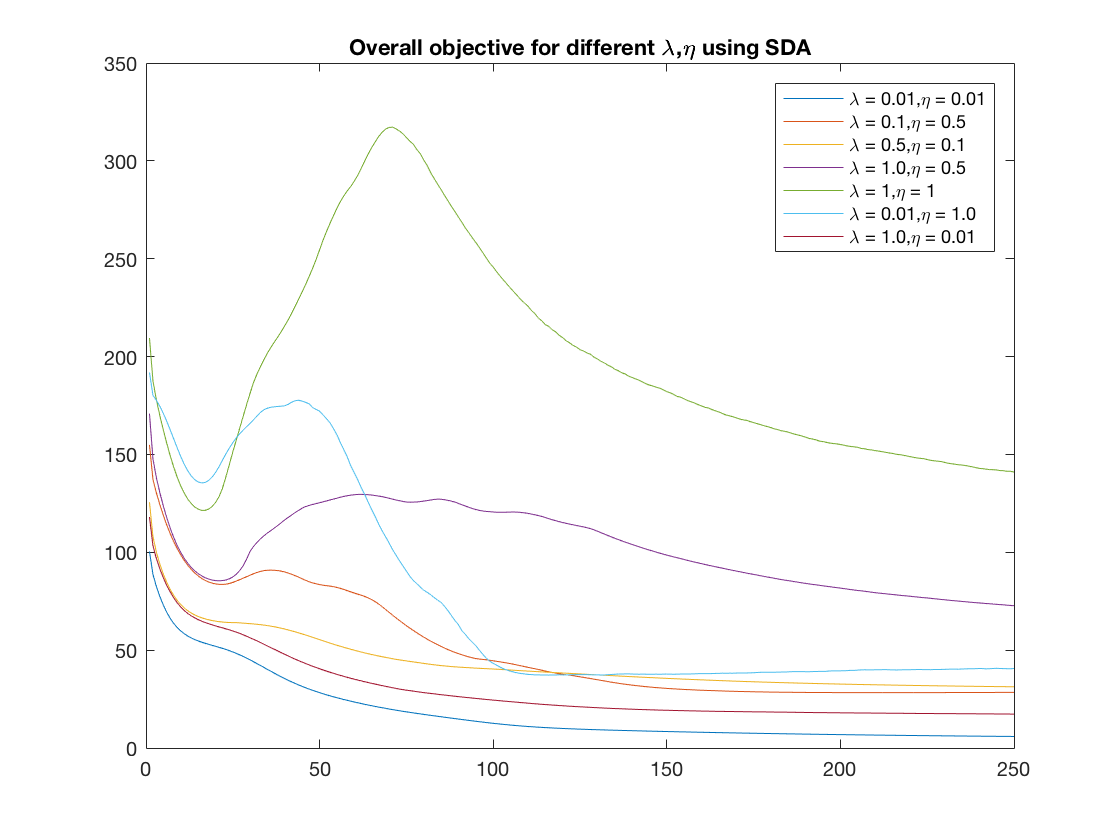
\includegraphics[scale=0.3]{SDA_overall}
  \end{subfigure}
\end{figure}
\end{center}
We see that the smallest objective is obtained at $\eta= 0.01,\lambda= 0.01$ -- this is no surprise as already discussed since the original matrix $\X$ was not obtained as a product of matrices which are sparse or smooth. We see that the smoothness constraint is what seems to hurt the overall objective the most and might be the reason why we see a peak of the objective around the $100$ iteration of the alternating minimization. We also see that the sparsity constraint does not hurt the objective too much. To compare the rank of $\Theta$ we recover for $\lambda = 1,\eta = 0.01$ is 32 while when $\lambda = 0.01,\eta = 0.01$ it is 37. To remind the reader the rank of $\X$ is 18. The next figures show how the objective decreases at each alternating minimization step of $200/500$ iterations for different values of $\lambda,\eta$. In each figure we plot how the objective in~\ref{problem_5} changes for a complete run of the SDA procedure to solve problem~\ref{problem_6},\ref{problem_7} or \ref{problem_8}. We do this for the first $25$ and the last $25$ calls to the SDA algorithm. The objective value is only computed every $10$ iterations.
\begin{center}
  \begin{figure}[H]
    \centering
  \begin{subfigure}[b]{0.3\textwidth}
    \includegraphics[scale=0.12]{{SDA_H_0.01_0.01}.png}
  \end{subfigure}
  \centering
  \begin{subfigure}[b]{0.3\textwidth}
    \includegraphics[scale=0.12]{{SDA_H_0.5_0.1}.png}
  \end{subfigure}
  \centering
  \begin{subfigure}[b]{0.3\textwidth}
    \includegraphics[scale=0.12]{{SDA_H_0.1_0.5}.png}
  \end{subfigure}
  \centering
  \begin{subfigure}[b]{0.3\textwidth}
    \includegraphics[scale=0.12]{{SDA_H_0.01_0.01last}.png}
  \end{subfigure}
  \centering
  \begin{subfigure}[b]{0.3\textwidth}
    \includegraphics[scale=0.12]{{SDA_H_0.5_0.1last}.png}
  \end{subfigure}
  \centering
  \begin{subfigure}[b]{0.3\textwidth}
    \includegraphics[scale=0.12]{{SDA_H_0.1_0.5last}.png}
  \end{subfigure}
  \caption{Plots of the overall objective as problem~\ref{problem_8} is being solved by SDA}
  \label{fig:SDA_H}
  \end{figure}
\end{center}
In figure~\ref{fig:SDA_H} we show the objective as $\H$ is being optimized over. As it is evident from the plots the objective does not change too much with $\H$ for later calls to SDA. This is consistent with the $\mathcal{O}(\frac{1}{\epsilon^2})$ convergence rate as the constant (by constant we refer to the quantity $D + \frac{k_g^2}{2}$ in the proof of Theorem 1.17 in lecture slides 4) depends on the norm of the gradient of problem~\ref{problem_8} (as already discussed) which in this case is around $900$.
\begin{center}
  \begin{figure}[h]
    \centering
  \begin{subfigure}[b]{0.3\textwidth}
    \includegraphics[scale=0.12]{{SDA_Th_0.01_0.01}.png}
  \end{subfigure}
  \centering
  \begin{subfigure}[b]{0.3\textwidth}
    \includegraphics[scale=0.12]{{SDA_Th_0.5_0.1}.png}
  \end{subfigure}
  \centering
  \begin{subfigure}[b]{0.3\textwidth}
    \includegraphics[scale=0.12]{{SDA_Th_0.1_0.5}.png}
  \end{subfigure}
  \centering
  \begin{subfigure}[b]{0.3\textwidth}
    \includegraphics[scale=0.12]{{SDA_Th_0.01_0.01last}.png}
  \end{subfigure}
  \centering
  \begin{subfigure}[b]{0.3\textwidth}
    \includegraphics[scale=0.12]{{SDA_Th_0.5_0.1last}.png}
  \end{subfigure}
  \centering
  \begin{subfigure}[b]{0.3\textwidth}
    \includegraphics[scale=0.12]{{SDA_Th_0.1_0.5last}.png}
  \end{subfigure}
  \caption{Plots of the overall objective as problem~\ref{problem_7} is being solved by SDA}
  \label{fig:SDA_Th}
  \end{figure}
\end{center}
Figure~\ref{fig:SDA_Th} contains similar experiments for $\Theta$, however, we observe something interesting -- unlike for $\H$ we see that at each consecutive call to SDA in the alternating minimization algorithm the objective for $\Theta$ goes up. This as a whole should not be a surprise as the objective in~\ref{problem_5} is not jointly convex in $\Theta,\H$ and $\W$ so we do not expect that an alternating minimization approach is always going to decrease the objective at each call. The more interesting observation here is the rate at which the objective decreases in the SDA algorithm -- it looks like it almost decreases at a linear rate which is unexpected as the theory suggest it should have sublinear behavior. One can argue that this might be related to the constant in the $\mathcal{O}(\frac{1}{\epsilon^2})$ being small for~\ref{problem_7} -- from our experiments it is around $120$.
\begin{center}
  \begin{figure}[H]
    \centering
  \begin{subfigure}[b]{0.3\textwidth}
    \includegraphics[scale=0.12]{{SDA_W_0.01_0.01}.png}
  \end{subfigure}
  \centering
  \begin{subfigure}[b]{0.3\textwidth}
    \includegraphics[scale=0.12]{{SDA_W_0.5_0.1}.png}
  \end{subfigure}
  \centering
  \begin{subfigure}[b]{0.3\textwidth}
    \includegraphics[scale=0.12]{{SDA_W_0.1_0.5}.png}
  \end{subfigure}
  \centering
  \begin{subfigure}[b]{0.3\textwidth}
    \includegraphics[scale=0.12]{{SDA_W_0.01_0.01last}.png}
  \end{subfigure}
  \centering
  \begin{subfigure}[b]{0.3\textwidth}
    \includegraphics[scale=0.12]{{SDA_W_0.5_0.1last}.png}
  \end{subfigure}
  \centering
  \begin{subfigure}[b]{0.3\textwidth}
    \includegraphics[scale=0.12]{{SDA_W_0.1_0.5last}.png}
  \end{subfigure}
  \caption{Plots of the overall objective as problem~\ref{problem_6} is being solved by SDA}
  \label{fig:SDA_W}
  \end{figure}
\end{center}
Finally in figure~\ref{fig:SDA_W} we show how the objective changes when solving~\ref{problem_6}. For early runs of SDA we see similar behavior to what is happening when solving~\ref{problem_8} with slightly faster convergence. This is within our expectations as the constant hidden in $\mathcal{O}(\frac{1}{\epsilon^2})$ is around $600$. For later applications (the last 25) we see behavior similar to~\ref{problem_7}. Our conjecture is that the norm of the gradients becomes much smaller as $\W_t$ approaches the overall optimal $\W^*$ and thus the constant $D+\frac{k_g^2}{2}$ since $D$ naturally decreases as $\W_t$ converges to $\W^*$.
\par
Even though we manage to get good performance in terms of convergence (compared to our best overall result) we still only use a small amount of iterations when solving each of the problems~\ref{problem_6},\ref{problem_7},\ref{problem_8} so we have no guarantees to be close to the optimal solution. To address this problem we run another two experiments in which the the number of iterations each SDA is ran for is $1000$ and $5000$. The number of iterations for the outer-most loop of the alternating optimization algorithm is still $250$. We only run these experiments for $\eta = 0.01$ and $\lambda = 0.01$ as they are very time-consuming.
\begin{centering}
  \begin{figure}[H]
    \includegraphics[scale = 0.3]{{SDA_overall1000}.png}
    \caption{Overall objective when SDA is ran for $1000$ iterations.}
    \label{fig:SDA_1000}
  \end{figure}
\end{centering}
The overall objective when SDA is ran for $1000$ iterations at each step is plotted in figure~\ref{fig:SDA_1000}. The best value achieved is $2.9022$. Comparing this to the best value achieved when SDA was ran for only $200$ iterations -- $5.8968$, it is better. In figure~\ref{fig:SDA_WTH1000} the individual runs are plotted for $\W$, $\Theta$ and $\H$.
\begin{center}
  \begin{figure}[H]
    \centering
  \begin{subfigure}[b]{0.3\textwidth}
    \includegraphics[scale=0.12]{{SDA_W_1000}.png}
  \end{subfigure}
  \centering
  \begin{subfigure}[b]{0.3\textwidth}
    \includegraphics[scale=0.12]{{SDA_H_1000}.png}
  \end{subfigure}
  \centering
  \begin{subfigure}[b]{0.3\textwidth}
    \includegraphics[scale=0.12]{{SDA_Th_1000}.png}
  \end{subfigure}
  \centering
  \begin{subfigure}[b]{0.3\textwidth}
    \includegraphics[scale=0.12]{{SDA_W_1000last}.png}
  \end{subfigure}
  \centering
  \begin{subfigure}[b]{0.3\textwidth}
    \includegraphics[scale=0.12]{{SDA_H_1000last}.png}
  \end{subfigure}
  \centering
  \begin{subfigure}[b]{0.3\textwidth}
    \includegraphics[scale=0.12]{{SDA_Th_1000last}.png}
  \end{subfigure}
  \caption{Plots of objective as $\W$, $\Theta$ and $\H$ are being optimized over with SDA for $1000$ iterations.}
  \label{fig:SDA_WTH1000}
  \end{figure}
\end{center}
All the plots look very similar to the ones where SDA is only ran for $200$ iterations in terms of how quickly the objective converges. The main difference seems to stem from the fact that after each individual call to SDA with $1000$ iterations the obtained solution has a slightly lower objective value compared to the SDA with $200$ iterations. These differences seem to diminish over the course of the $250$ iterations of the outer most loop and we conjecture that if we ran the outer loop for more than $250$ we would get about the same results. Comparing the run-time of both SDA with $200$ iterations and SDA with $1000$ iterations the gain is almost insignificant. We do not expect running SDA for $5000$ iterations per optimization problem is going to perform much better. The plots containing the experiments in which SDA is ran for $5000$ iterations can be seen in figures~\ref{fig:SDA_5000} and~\ref{fig:SDA_WTH5000}. The best value we get for the overall objective is $2.0425$.
\begin{centering}
  \begin{figure}[H]
    \includegraphics[scale = 0.3]{{SDA_overall5000}.png}
    \caption{Overall objective when SDA is ran for $5000$ iterations.}
    \label{fig:SDA_5000}
  \end{figure}
\end{centering}
\begin{center}
  \begin{figure}[H]
    \centering
  \begin{subfigure}[b]{0.3\textwidth}
    \includegraphics[scale=0.12]{{SDA_W_5000}.png}
  \end{subfigure}
  \centering
  \begin{subfigure}[b]{0.3\textwidth}
    \includegraphics[scale=0.12]{{SDA_H_5000}.png}
  \end{subfigure}
  \centering
  \begin{subfigure}[b]{0.3\textwidth}
    \includegraphics[scale=0.12]{{SDA_Th_5000}.png}
  \end{subfigure}
  \centering
  \begin{subfigure}[b]{0.3\textwidth}
    \includegraphics[scale=0.12]{{SDA_W_5000last}.png}
  \end{subfigure}
  \centering
  \begin{subfigure}[b]{0.3\textwidth}
    \includegraphics[scale=0.12]{{SDA_H_5000last}.png}
  \end{subfigure}
  \centering
  \begin{subfigure}[b]{0.3\textwidth}
    \includegraphics[scale=0.12]{{SDA_Th_5000last}.png}
  \end{subfigure}
  \caption{Plots of objective as $\W$, $\Theta$ and $\H$ are being optimized over with SDA for $5000$ iterations.}
  \label{fig:SDA_WTH5000}
  \end{figure}
\end{center}
For a final experiment on stopping criteria we ran SDA stopping the algorithm if the distance between two consecutive iterates became less than $10^{-4}$ (or since at early stages of the overall optimization procedure it took too many iterations we stopped it after the first $5000$ iterations). We noticed that after the first $50$ iterations of the overall alternating minimization procedure the SDA algorithm was stopping before the $5000$ iterations expired. The result for the overall objective at the end was $2.8784$ which is slightly better than just stopping SDA after $1000$ iterations and worse than stopping SDA after $5000$ iterations. This implies that stopping when iterates do not change too much between iterations is not enough to guarantee better overall performance. The only plot we provide~\ref{fig:SDA_STOP} is for the overall objective as the plots for the separate problems are almost identical to the ones for SDA with $1000$ iterations.
\par
To conclude this section -- we did not observe anything unexpected considering theory of convergence of SDA. The most surprising results were in the convergence speed of $\Theta$ but this can still be explained by the smaller distance between initialization and optimal $\Theta$ and smaller norm of the gradients for the objective. We also observed that for $\Theta$ and at later iterations of the alternating minimization procedure for $\W$ that a lot of computational work is wasted as each optimization subproblem starts almost at the same objective value as the previous.
\begin{center}
  \begin{figure}[H]
    \includegraphics[scale = 0.3]{{SDA_overall_early}.png}
    \caption{Overall objective when SDA is ran for $5000$ iterations.}
    \label{fig:SDA_STOP}
  \end{figure}
\end{center}

\section{Augmented Lagrangian}



\bibliographystyle{plain}
\bibliography{mybibfile}
\end{document}
